\begin{figure}[tp]
\definecolor{tak}{HTML}{d3e2ff}
\definecolor{vol}{HTML}{deffb0}
\definecolor{leeg}{HTML}{ffc5b7}
\definecolor{ongevuld}{rgb}{0.85, 0.85, 0.85}


\tikzstyle{array_element_0}=[rectangle,
                                            minimum size=5cm,
                                            draw=black,
                                            rounded corners=2.5 ]

\tikzstyle{array_element_1}=[rectangle,
                                            minimum size=2.5cm,
                                            draw=black,
                                            rounded corners=2.5 ]

\tikzstyle{array_element_2}=[rectangle,
                                              minimum size=1.25cm,
                                              draw=black,
                                              rounded corners=2.5 ]

\tikzstyle{array_element_3}=[rectangle,
                                              minimum size=0.625cm,
                                              draw=black,
                                              rounded corners=2.5 ]

\tikzstyle{n_element}=[circle,draw, minimum size=1cm, thick]

\tikzstyle{node_element}=[rectangle,
                                            minimum height=1.5cm, 
                                            minimum width=1.5cm, 
                                            minimum size=0.75cm,
                                            draw=black,
                                            rounded corners=2.5 ]
                                            
\tikzstyle{phi_element}=[rectangle,
                                            minimum height=1.5cm, 
                                            minimum width=1.5cm, 
                                            minimum size=1.25cm,
                                            draw=black,
                                            rounded corners=2.5 ]

\hspace{0.05\textwidth}
\begin{adjustbox}{minipage=\textwidth, scale=0.5}
  \centering
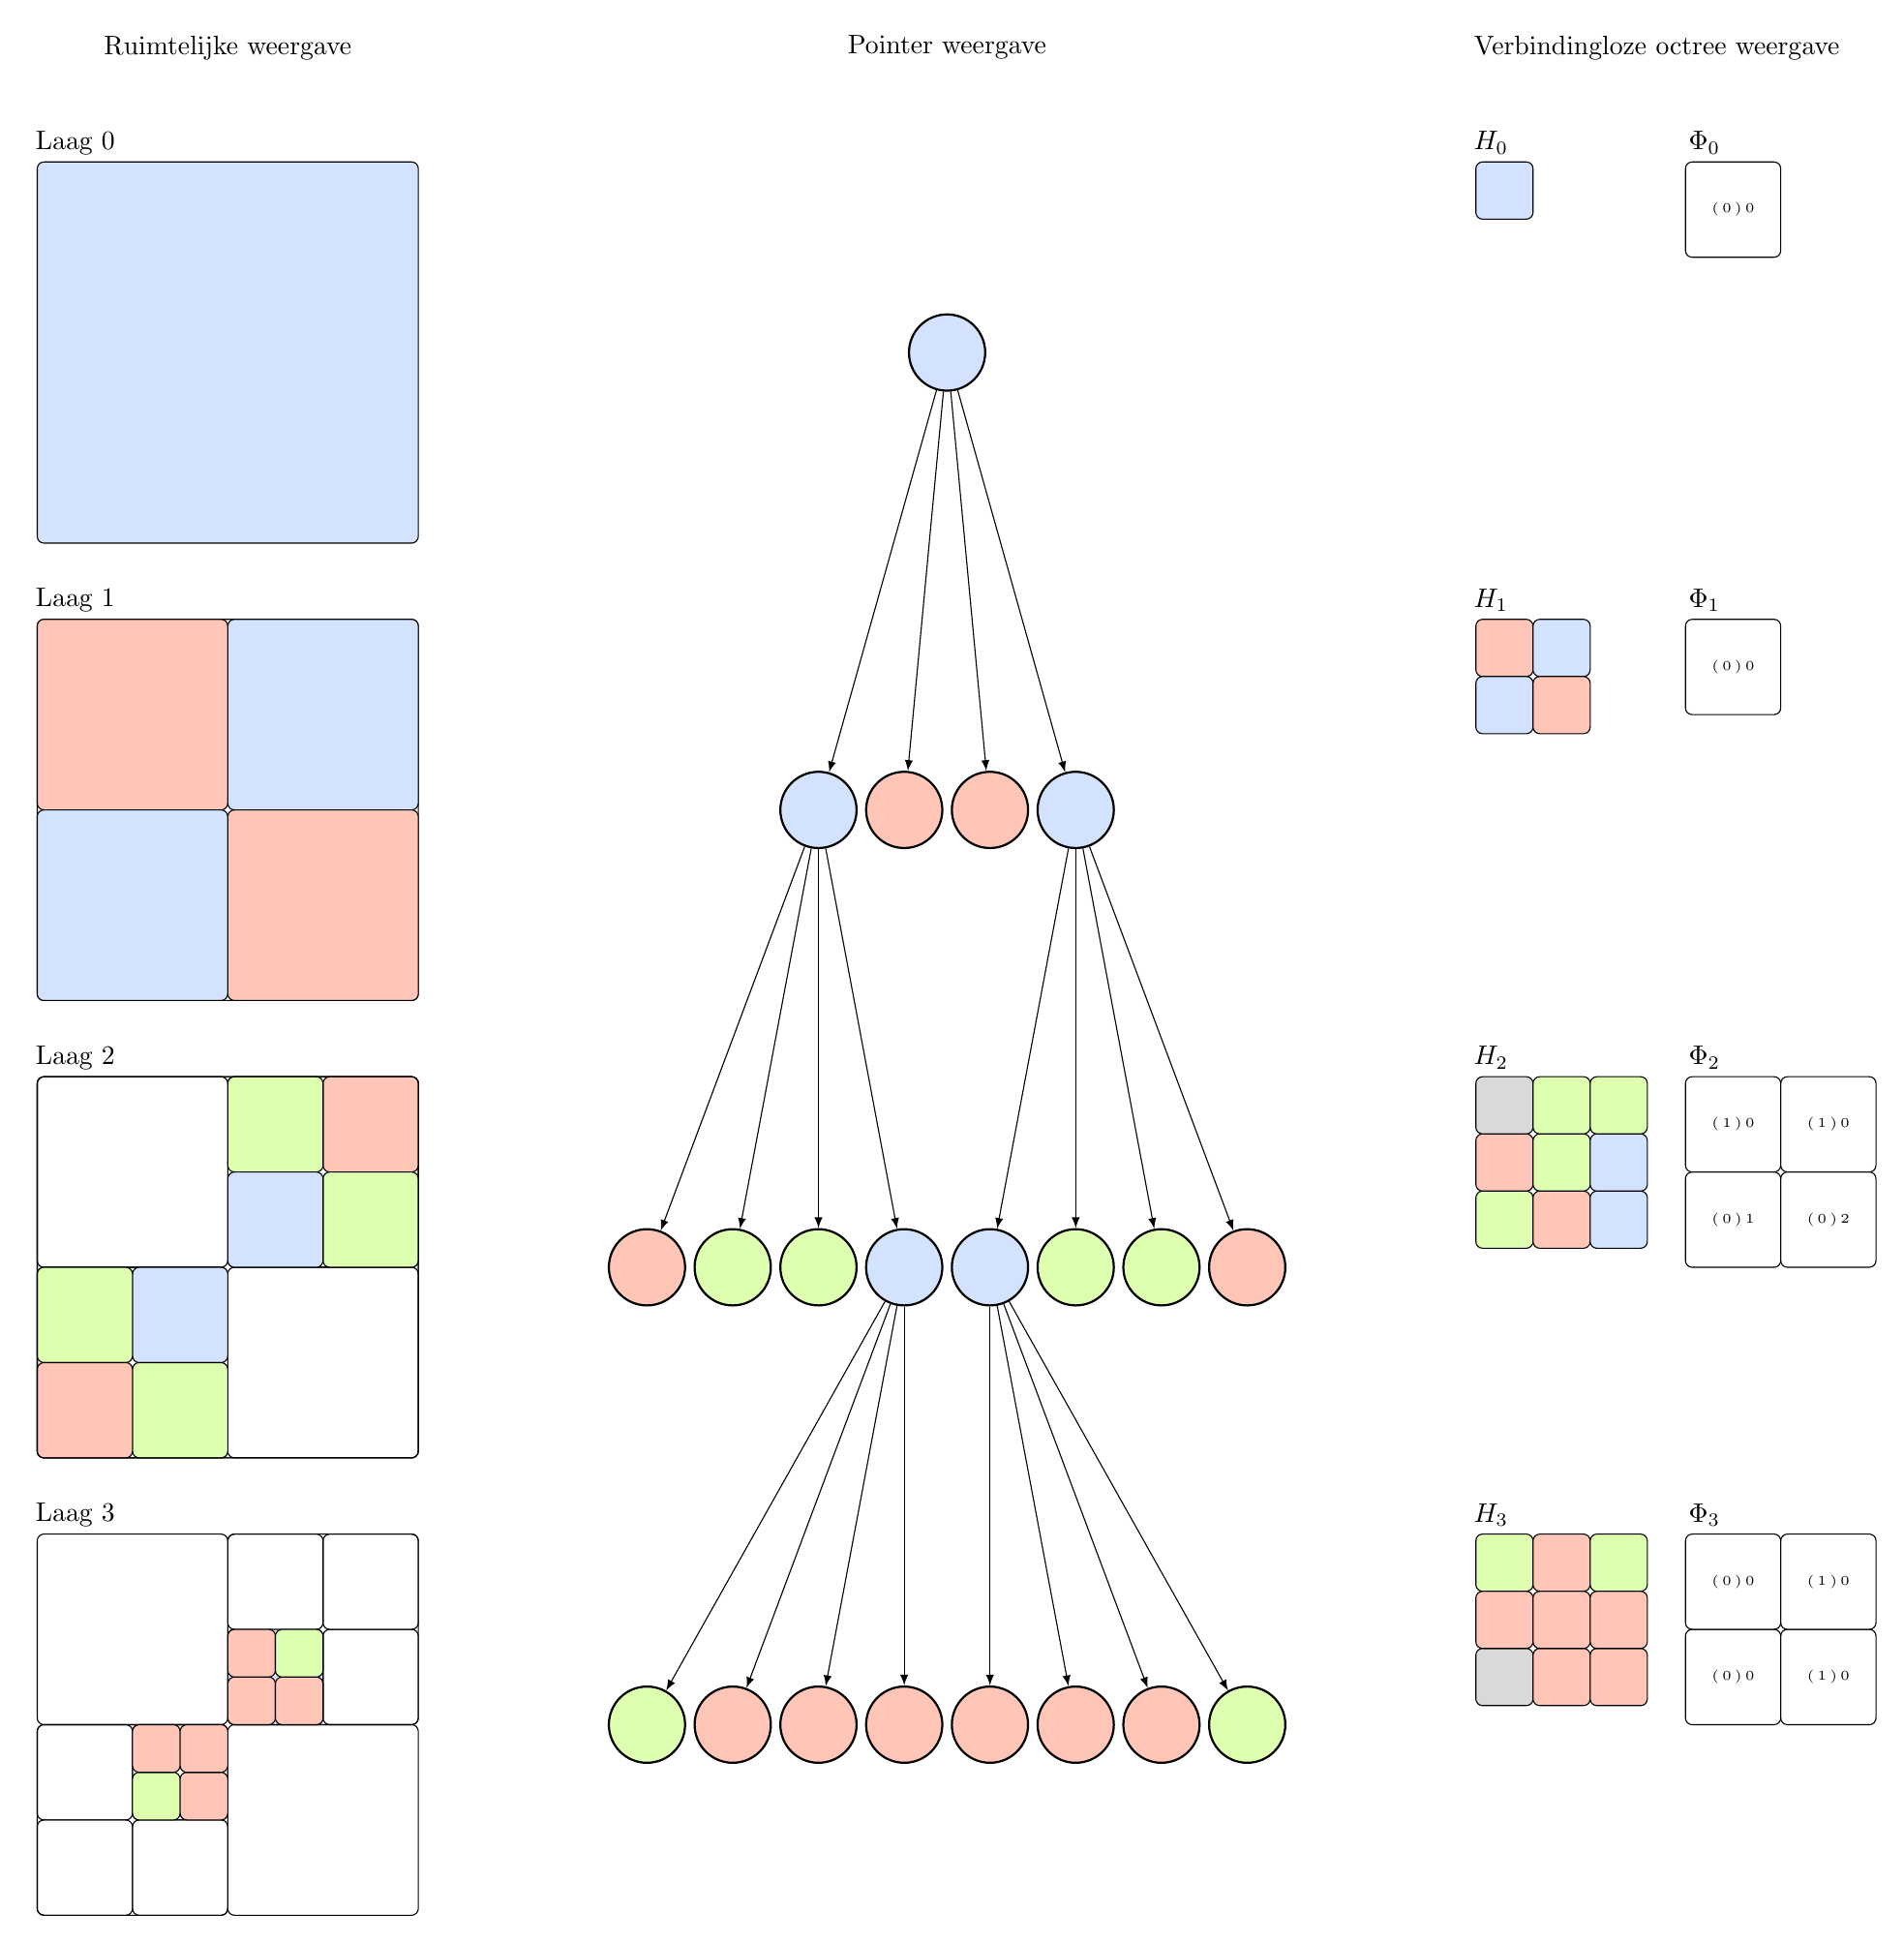
\begin{tikzpicture}
 % laag 0
 % -------------------------------------------------------------------------------
  \node at (0cm, 12cm) (n0) [array_element_0, fill=tak]  {};

 % laag 1
 % -------------------------------------------------------------------------------
  \node at (0cm, 6cm) (n0) [array_element_0]  {};
  \node at (-1.25cm, 7.25cm) (n0) [array_element_1, fill=leeg]  {};
  \node at ( 1.25cm, 7.25cm) (n0) [array_element_1, fill=tak]  {};
  \node at (-1.25cm, 4.75cm) (n0) [array_element_1, fill=tak]  {};
  \node at ( 1.25cm, 4.75cm) (n0) [array_element_1, fill=leeg]  {};

 % laag 2
 % -------------------------------------------------------------------------------
  \node at (0cm, 0cm) (n0) [array_element_0]  {};
  \node at (-1.25cm,  1.25cm) (n0) [array_element_1]  {};
  \node at ( 1.25cm,   1.25cm) (n0) [array_element_1] {};
  \node at (-1.25cm, -1.25cm) (n0) [array_element_1] {};
  \node at ( 1.25cm, -1.25cm) (n0) [array_element_1] {};
   
  \node at (1.25cm + 0.625cm, 1.25cm + 0.625cm) (n0) [array_element_2, fill=leeg]  {};
  \node at (1.25cm - 0.625cm, 1.25cm + 0.625cm) (n0) [array_element_2, fill=vol]  {};
  \node at (1.25cm + 0.625cm, 1.25cm - 0.625cm) (n0) [array_element_2, fill=vol]  {};
  \node at (1.25cm - 0.625cm, 1.25cm - 0.625cm) (n0) [array_element_2, fill=tak]  {};

  \node at (-1.25cm + 0.625cm, -1.25cm + 0.625cm) (n0) [array_element_2, fill=tak]  {};
  \node at (-1.25cm - 0.625cm, -1.25cm + 0.625cm) (n0) [array_element_2, fill=vol]  {};
  \node at (-1.25cm + 0.625cm, -1.25cm - 0.625cm) (n0) [array_element_2, fill=vol]  {};
  \node at (-1.25cm - 0.625cm, -1.25cm - 0.625cm) (n0) [array_element_2, fill=leeg]  {};

  % laag 3
  % -------------------------------------------------------------------------------
    \node at (0cm, 0cm) (n0) [array_element_0]  {};
  \node at (-1.25cm,  1.25cm - 6cm) (n0) [array_element_1]  {};
  \node at ( 1.25cm,   1.25cm - 6cm) (n0) [array_element_1] {};
  \node at (-1.25cm, -1.25cm - 6cm) (n0) [array_element_1] {};
  \node at ( 1.25cm, -1.25cm - 6cm) (n0) [array_element_1] {};
   
  \node at (1.25cm + 0.625cm, 1.25cm + 0.625cm - 6cm) (n0) [array_element_2]  {};
  \node at (1.25cm - 0.625cm, 1.25cm + 0.625cm - 6cm) (n0) [array_element_2]  {};
  \node at (1.25cm + 0.625cm, 1.25cm - 0.625cm - 6cm) (n0) [array_element_2]  {};
  \node at (1.25cm - 0.625cm, 1.25cm - 0.625cm - 6cm) (n0) [array_element_2, fill=tak]  {};

  \node at (-1.25cm + 0.625cm, -1.25cm + 0.625cm - 6cm) (n0) [array_element_2]  {};
  \node at (-1.25cm - 0.625cm, -1.25cm + 0.625cm - 6cm) (n0) [array_element_2]  {};
  \node at (-1.25cm + 0.625cm, -1.25cm - 0.625cm - 6cm) (n0) [array_element_2]  {};
  \node at (-1.25cm - 0.625cm, -1.25cm - 0.625cm - 6cm) (n0) [array_element_2]  {};

  \node at (-1.25cm + 0.625cm - 0.3125cm, -1.25cm + 0.625cm - 6cm -0.3125cm) (n0) [array_element_3, fill=vol]  {};
  \node at (-1.25cm + 0.625cm + 0.3125cm, -1.25cm + 0.625cm - 6cm -0.3125cm) (n0) [array_element_3, fill=leeg]  {};
  \node at (-1.25cm + 0.625cm - 0.3125cm, -1.25cm + 0.625cm - 6cm + 0.3125cm) (n0) [array_element_3, fill=leeg]  {};
  \node at (-1.25cm + 0.625cm + 0.3125cm, -1.25cm + 0.625cm - 6cm + 0.3125cm) (n0) [array_element_3, fill=leeg]  {};

  \node at (1.25cm - 0.625cm - 0.3125cm, 1.25cm - 0.625cm - 6cm -0.3125cm) (n0) [array_element_3, fill=leeg]  {};
  \node at (1.25cm - 0.625cm + 0.3125cm, 1.25cm - 0.625cm - 6cm -0.3125cm) (n0) [array_element_3, fill=leeg]  {};
  \node at (1.25cm - 0.625cm - 0.3125cm, 1.25cm - 0.625cm - 6cm + 0.3125cm) (n0) [array_element_3, fill=leeg]  {};
  \node at (1.25cm - 0.625cm + 0.3125cm, 1.25cm - 0.625cm - 6cm + 0.3125cm) (n0) [array_element_3, fill=vol]  {};
  
  \node at (5.5cm + 3.5 * 1.125cm, 12cm) (v00) [n_element, fill=tak] {};

  \node at (5.5cm + 2 * 1.125cm, 6cm) (v10) [n_element, fill=tak] {};
  \node at (5.5cm + 3 * 1.125cm, 6cm) (v11) [n_element, fill=leeg] {};
  \node at (5.5cm + 4 * 1.125cm, 6cm) (v12) [n_element, fill=leeg] {};
  \node at (5.5cm + 5 * 1.125cm, 6cm) (v13) [n_element, fill=tak] {};

  \node at (5.5cm + 0 * 1.125cm, 0cm) (v20) [n_element, fill=leeg] {};
  \node at (5.5cm + 1 * 1.125cm, 0cm) (v21) [n_element, fill=vol] {};
  \node at (5.5cm + 2 * 1.125cm, 0cm) (v22) [n_element, fill=vol] {};
  \node at (5.5cm + 3 * 1.125cm, 0cm) (v23) [n_element, fill=tak] {};
  \node at (5.5cm + 4 * 1.125cm, 0cm) (v24) [n_element, fill=tak] {};
  \node at (5.5cm + 5 * 1.125cm, 0cm) (v25) [n_element, fill=vol] {};
  \node at (5.5cm + 6 * 1.125cm, 0cm) (v26) [n_element, fill=vol] {};
  \node at (5.5cm + 7 * 1.125cm, 0cm) (v27) [n_element, fill=leeg] {};

  \node at (5.5cm + 0 * 1.125cm, -6cm) (v30) [n_element, fill=vol] {};
  \node at (5.5cm + 1 * 1.125cm, -6cm) (v31) [n_element, fill=leeg] {};
  \node at (5.5cm + 2 * 1.125cm, -6cm) (v32) [n_element, fill=leeg] {};
  \node at (5.5cm + 3 * 1.125cm, -6cm) (v33) [n_element, fill=leeg] {};
  \node at (5.5cm + 4 * 1.125cm, -6cm) (v34) [n_element, fill=leeg] {};
  \node at (5.5cm + 5 * 1.125cm, -6cm) (v35) [n_element, fill=leeg] {};
  \node at (5.5cm + 6 * 1.125cm, -6cm) (v36) [n_element, fill=leeg] {};
  \node at (5.5cm + 7 * 1.125cm, -6cm) (v37) [n_element, fill=vol] {};
  
  \foreach \a in {0, ..., 3} {
    \draw[-latex] (v00) -- (v1\a);
  }
\foreach \a in {0, ..., 3} {
    \draw[-latex] (v10) -- (v2\a);
  }
\foreach \a in {4, ..., 7} {
    \draw[-latex] (v13) -- (v2\a);
  }

\foreach \a in {0, ..., 3} {
    \draw[-latex] (v23) -- (v3\a);
  }
\foreach \a in {4, ..., 7} {
    \draw[-latex] (v24) -- (v3\a);
  }

\node at (16.75cm, 14.5cm - 0.375cm) (UC1) [node_element, fill=tak] {};
\node at (19.75cm, 14.5cm - 0.625cm) (UC1) [phi_element] {\tiny $\begin{pmatrix}0\\0\end{pmatrix}$};

% ----------------------
\node at (16.75cm, 8.5cm - 0.375cm) (UC1) [node_element, fill=leeg] {};
\node at (16.75cm + 0.75cm, 8.5cm - 0.375cm) (UC1) [node_element, fill=tak] {};
\node at (16.75cm, 8.5cm - 0.375cm - 0.75cm) (UC1) [node_element, fill=tak] {};
\node at (16.75cm + 0.75cm, 8.5cm - 0.375cm- 0.75cm) (UC1) [node_element, fill=leeg] {};
\node at (19.75cm, 8.5cm - 0.625cm) (UC1) [phi_element] {\tiny $\begin{pmatrix}0\\0\end{pmatrix}$};

% ------------

\node at (16.75cm + 0 * 0.75cm, 2.5cm - 0.375cm  - 2 * 0.75cm) (UC1) [node_element, fill=vol] {};
\node at (16.75cm + 1 * 0.75cm, 2.5cm - 0.375cm  - 2 * 0.75cm) (UC1) [node_element, fill=leeg] {};
\node at (16.75cm + 2 * 0.75cm, 2.5cm - 0.375cm  - 2 * 0.75cm) (UC1) [node_element, fill=tak] {};

\node at (16.75cm + 0 * 0.75cm, 2.5cm - 0.375cm  - 1 * 0.75cm) (UC1) [node_element, fill=leeg] {};
\node at (16.75cm + 1 * 0.75cm, 2.5cm - 0.375cm  - 1 * 0.75cm) (UC1) [node_element, fill=vol] {};
\node at (16.75cm + 2 * 0.75cm, 2.5cm - 0.375cm  - 1 * 0.75cm) (UC1) [node_element, fill=tak] {};

\node at (16.75cm + 0 * 0.75cm, 2.5cm - 0.375cm  - 0 * 0.75cm) (UC1) [node_element, fill=ongevuld] {};
\node at (16.75cm + 1 * 0.75cm, 2.5cm - 0.375cm  - 0 * 0.75cm) (UC1) [node_element, fill=vol] {};
\node at (16.75cm + 2 * 0.75cm, 2.5cm - 0.375cm  - 0 * 0.75cm) (UC1) [node_element, fill=vol] {};


\node at (19.75cm, 2.5cm - 0.625cm - 1.25cm) (UC1) [phi_element] {\tiny $\begin{pmatrix}0\\1\end{pmatrix}$};
\node at (19.75cm + 1.25cm, 2.5cm - 0.625cm - 1.25cm) (UC1) [phi_element] {\tiny $\begin{pmatrix}0\\2\end{pmatrix}$};
\node at (19.75cm, 2.5cm - 0.625cm) (UC1) [phi_element] {\tiny $\begin{pmatrix}1\\0\end{pmatrix}$};
\node at (19.75cm + 1.25cm, 2.5cm - 0.625cm) (UC1) [phi_element] {\tiny $\begin{pmatrix}1\\0\end{pmatrix}$};


% -------------------------
\node at (16.75cm + 0 * 0.75cm, 2.5cm - 0.375cm  - 2 * 0.75cm -6cm) (UC1) [node_element, fill=ongevuld] {};
\node at (16.75cm + 1 * 0.75cm, 2.5cm - 0.375cm  - 2 * 0.75cm -6cm) (UC1) [node_element, fill=leeg] {};
\node at (16.75cm + 2 * 0.75cm, 2.5cm - 0.375cm  - 2 * 0.75cm -6cm) (UC1) [node_element, fill=leeg] {};


\node at (16.75cm + 0 * 0.75cm, 2.5cm - 0.375cm  - 1 * 0.75cm -6cm) (UC1) [node_element, fill=leeg] {};
\node at (16.75cm + 1 * 0.75cm, 2.5cm - 0.375cm  - 1 * 0.75cm -6cm) (UC1) [node_element, fill=leeg] {};
\node at (16.75cm + 2 * 0.75cm, 2.5cm - 0.375cm  - 1 * 0.75cm -6cm) (UC1) [node_element, fill=leeg] {};


\node at (16.75cm + 0 * 0.75cm, 2.5cm - 0.375cm  - 0 * 0.75cm -6cm) (UC1) [node_element, fill=vol] {};
\node at (16.75cm + 1 * 0.75cm, 2.5cm - 0.375cm  - 0 * 0.75cm -6cm) (UC1) [node_element, fill=leeg] {};
\node at (16.75cm + 2 * 0.75cm, 2.5cm - 0.375cm  - 0 * 0.75cm -6cm) (UC1) [node_element, fill=vol] {};

\node at (19.75cm, 2.5cm - 0.625cm - 1.25cm -6cm) (UC1) [phi_element] {\tiny $\begin{pmatrix}0\\0\end{pmatrix}$};
\node at (19.75cm + 1.25cm, 2.5cm - 0.625cm - 1.25cm -6cm) (UC1) [phi_element] {\tiny $\begin{pmatrix}1\\0\end{pmatrix}$};
\node at (19.75cm, 2.5cm - 0.625cm -6cm) (UC1) [phi_element] {\tiny $\begin{pmatrix}0\\0\end{pmatrix}$};
\node at (19.75cm + 1.25cm, 2.5cm - 0.625cm -6cm) (UC1) [phi_element] {\tiny $\begin{pmatrix}1\\0\end{pmatrix}$};


\node (l1) at (-2.cm, 14.75cm) {Laag 0};
\node (l1) at (-2.cm, 8.75cm) {Laag 1};
\node (l1) at (-2.cm, 2.75cm) {Laag 2};
\node (l1) at (-2.cm, -3.25cm) {Laag 3};

\node (l1) at (0cm, 16cm) {Ruimtelijke weergave};
\node (l1) at (5.5cm + 3.5 * 1.125cm, 16cm) {Pointer weergave};
\node (l1) at (18.75cm, 16cm) {Verbindingloze octree weergave};

\node (l1) at (16.575cm, 14.75cm) {$H_0$};
\node (l1) at (19.375cm, 14.75cm) {$\Phi_0$};

\node (l1) at (16.575cm, 14.75cm  - 1 * 6cm) {$H_1$};
\node (l1) at (19.375cm, 14.75cm  - 1 * 6cm) {$\Phi_1$};

\node (l1) at (16.575cm, 14.75cm  - 2 * 6cm) {$H_2$};
\node (l1) at (19.375cm, 14.75cm  - 2 * 6cm) {$\Phi_2$};

\node (l1) at (16.575cm, 14.75cm  - 3 * 6cm) {$H_3$};
\node (l1) at (19.375cm, 14.75cm  - 3 * 6cm) {$\Phi_3$};


\end{tikzpicture}
\end{adjustbox}
  \caption{Een voorbeeld van de representatie van een octree met behulp van een verbindingloze octree.}
  \label{fig:hs-linkless-octree-representation}
\end{figure}
